% !TeX root = ..\rapport_13_1.tex
\section{Kravspecifikation}
\subsection{Indledning}
Denne del af eksamensopgaven dokumenterer vores planlægningsproces, der skal tilvejebringe et tids/projektstyringsprogram der møder Softwarehuset A/S' ønsker. Det gøres ved hjælp af ideer og modeller fra Behavior- og Test Driven Development, der ved hjælp af brainstorming lader os gå fra kundeønsker til scenarier, fra scenarier til tests og fra tests til kode (tests og kode i næste rapport), alt sammen med rod i beskrivelsen af Softwarehusets ønsker.
\subsection{Ordliste}
\begin{table}[H]
    \centering
    \setlength{\extrarowheight}{8pt}
    \begin{tabular}{>{\bfseries}l p{0.73\textwidth}}
        Medarbejder           & \textit{[Employee]} En medarbejder er en person ansat i Softwarehuset A/S, som er tildelt aktiviteter. En medarbejder kan udføre aktiviteter og registrere arbejdstid brugt på aktiviteter, uagtet om medarbejderen er tilknyttet aktiviteten. Hver medarbejder har et medarbejder ID.                                         \\
        Projekt aktivitet     & \textit{[Project activity]} En delopgave af et projekt. Hver aktivitet er tilknyttet en medarbejder.                                                                                                                                                                                                                           \\
        Fast aktivitet        & \textit{[Regular activity]} Aktivitet der ikke kan pålægges et projekt. F.eks. ferie, sygdom, kurser.                                                                                                                                                                                                                          \\
        Projekt               & \textit{[Project]} Udviklingsarbejde udført for en kunde (eksternt) eller for Softwarehuset A/S (internt). Et projekt administreres af en projektleder og er inddelt i aktiviteter. Hvert projekt har et projektnummer.                                                                                                        \\
        Kunde                 & \textit{[Customer]} En ekstern entitet som bestiller og er modtager af projekter.                                                                                                                                                                                                                                              \\
        Projektleder          & \textit{[Project leader]} En medarbejder der har ret til at oprette og tildele aktiviteter for et givent projekt.                                                                                                                                                                                                              \\
        Softwarehuset A/S     & \textit{[Softwarehuset A/S]} Entitet som er modtager af et projekt, hvis projektet er internt.                                                                                                                                                                                                                                 \\
        Medarbejder initialer & \textit{[Employee initials]} Unik identifikation for hver enkelt medarbejder, bestående af fire bogstaver. To første fra fornavn efterfulgt af to første fra efternavn. F.eks. ``rawi''. Hvis initialer allerede er taget, vælges bogstav et og tre i efternavn, derefter et og fire, osv.                                     \\
        Projektnummer         & \textit{[Project number]} Identifikation for hvert enkelt projekt. Har formen årstal efterfulgt af et trecifret løbenummer. F.eks. 23001                                                                                                                                                                                      \\
        Budgetteret tid       & \textit{[Time budget]} En aktivitets estimerede antal hele timer.                                                                                                                                                                                                                                                              \\
        Arbejdstid            & \textit{[Work time]} Mængde tid i inkrementer af halve timer, brugt på en aktivitet. Kan registreres af den medarbejder som har brugt arbejdstid på en given aktivitet.                                                                                                                                                        \\
        Start- og sluttid     & \textit{[start- and end week]} En periode med opløsning på uge-niveau til aktiviteter. Begge tider angives som år og uge, ved formatet ``ÅÅUU''. F.eks. 2304 for uge 4 i 2023. En starttid afgrænser starten af en given uge, en sluttid afgrænser ved slutningen af en given uge. Start- og sluttid kan derfor godt være ens.
    \end{tabular}
\end{table}\newpage
\subsection{Use case diagrammer}
Dette afsnit starter med \cref{fig:AlleActorsPaaEnGang} som viser hvilke aktører der kan udfører hvilke cases. Herefter kommer en oversigt (\cref{tbl:oversigt}) over de detaljerede use cases og hvilke sider der indeholder Cucumber features (\cpagerefrange{lst:usecase_register_employee}{lst:remainingTime}) og sekvensdiagrammer (\cref{sec:sequence}).
\begin{figure}[H]
    \centering
    \caption{Use case diagram for programmet hvori de tre aktører inkluderet er Gæst, Medarbejder og Projektleder.}\label{fig:AlleActorsPaaEnGang}
    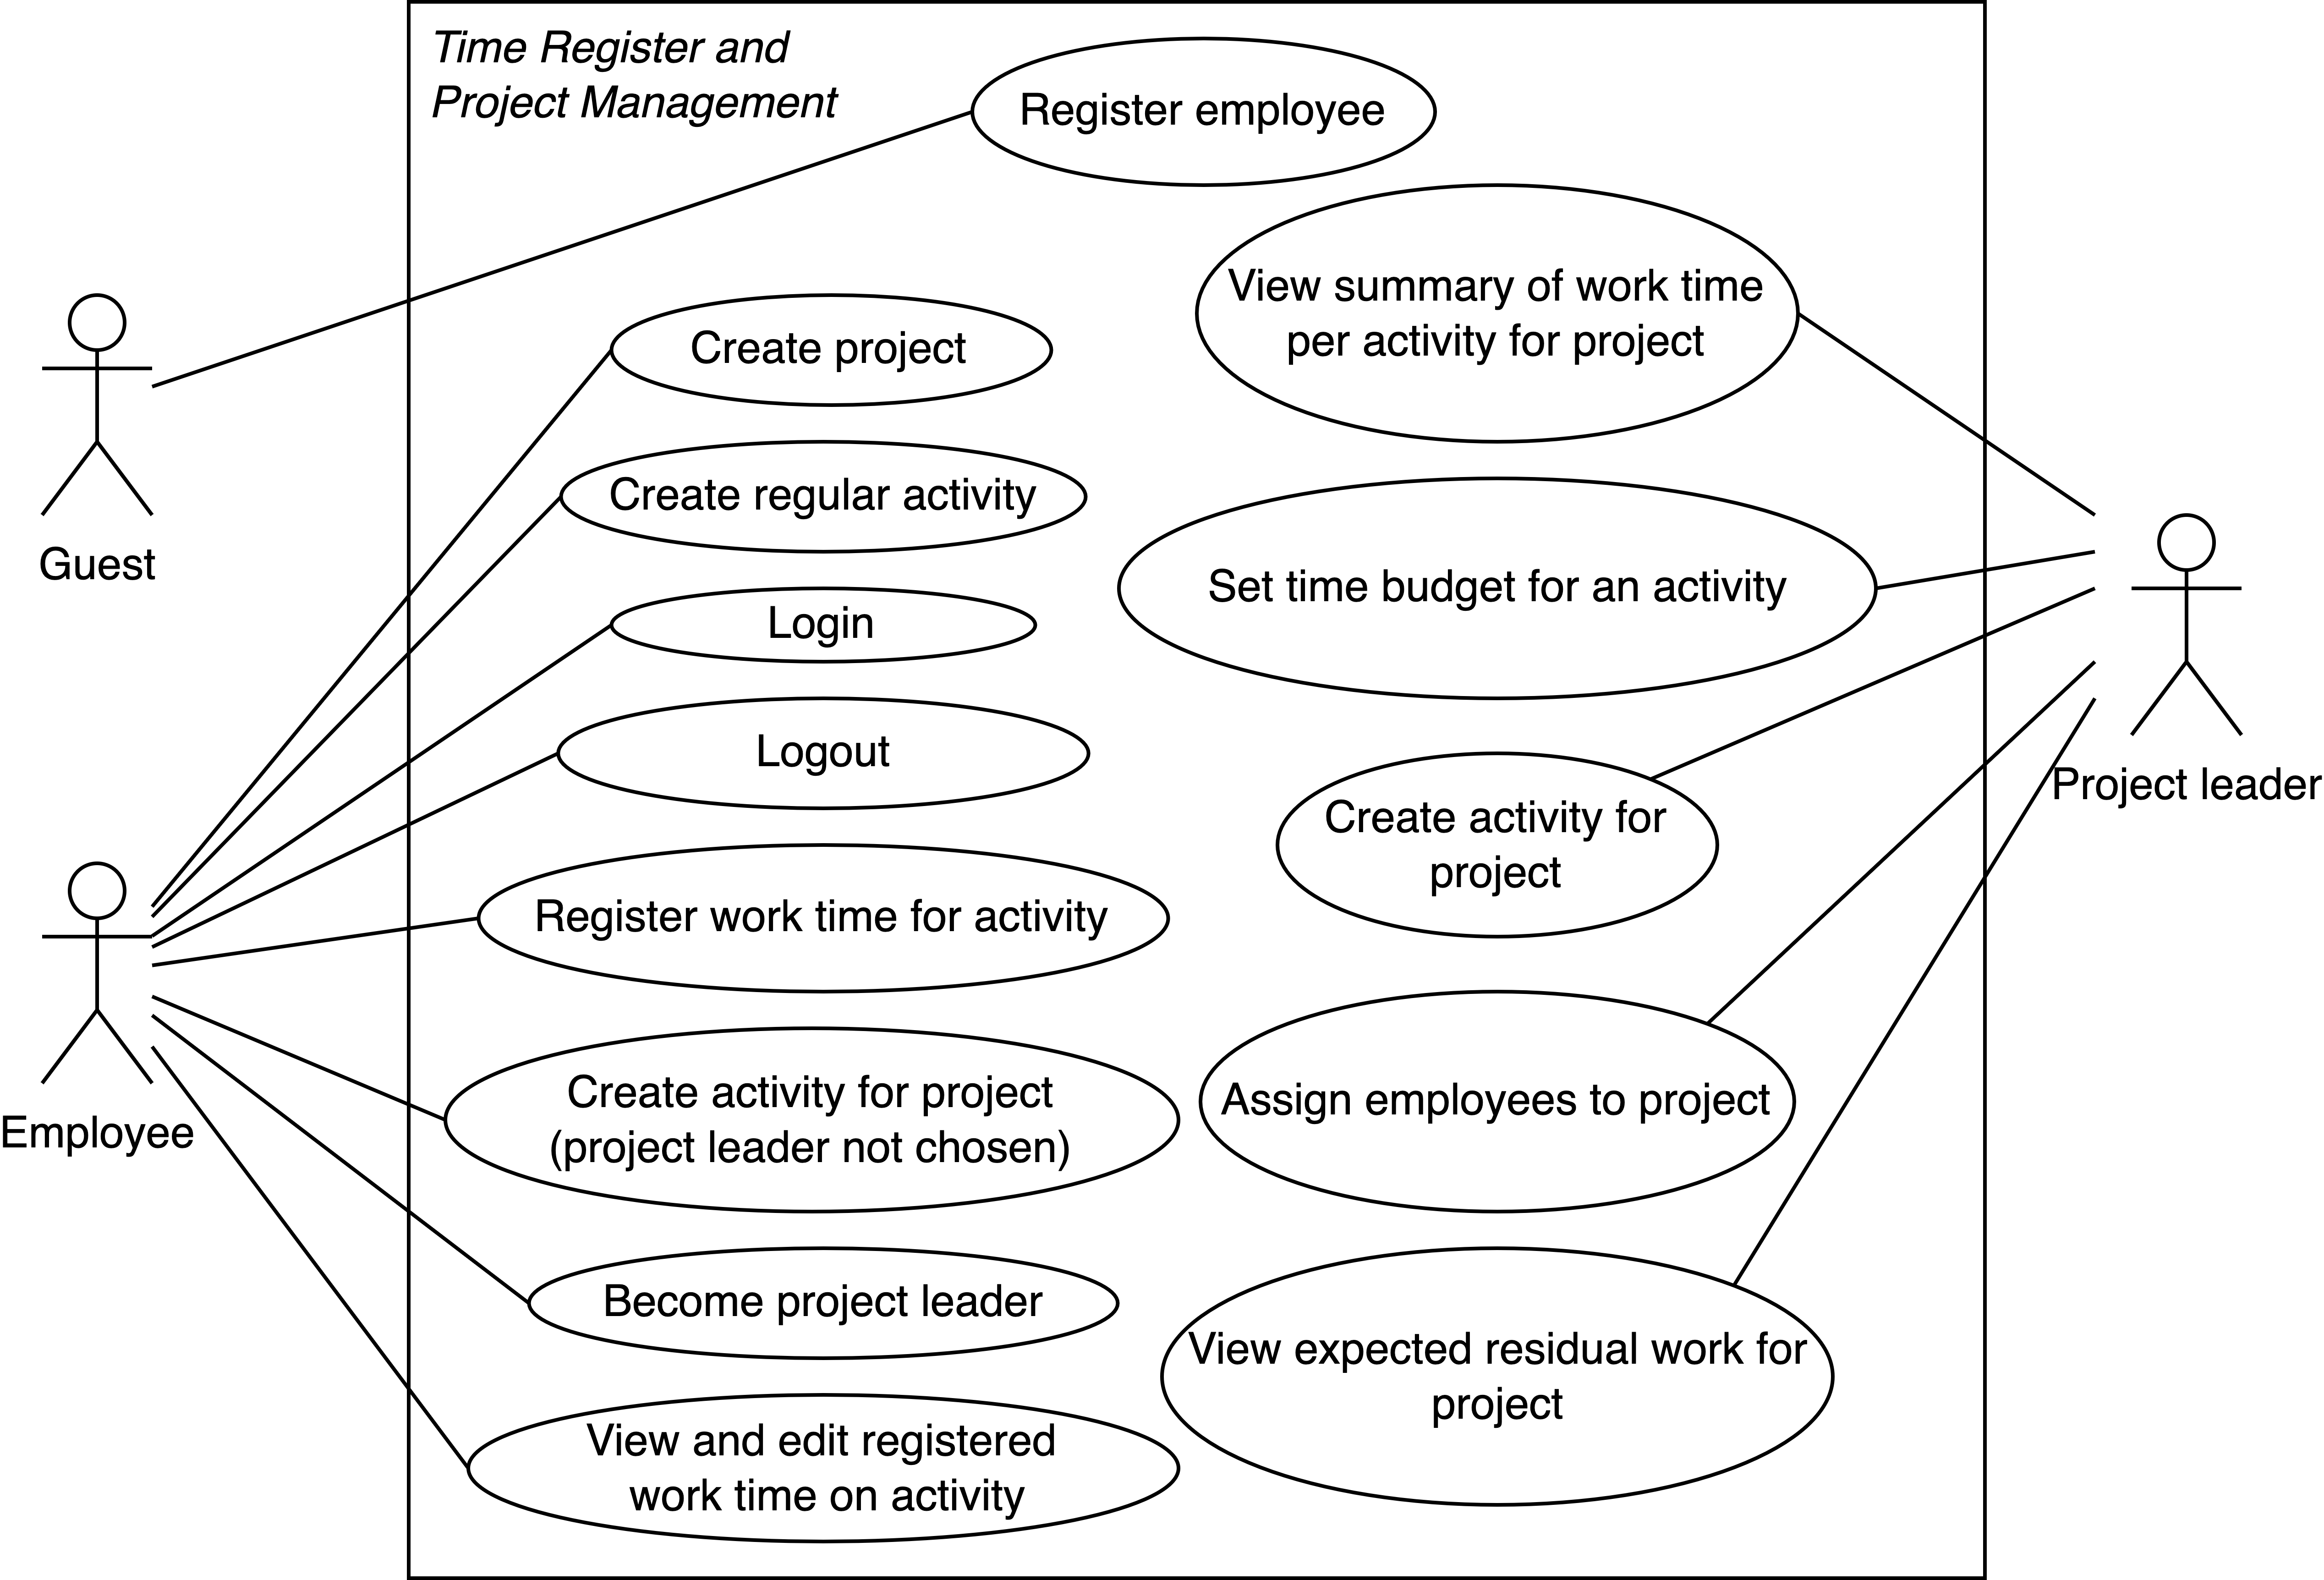
\includegraphics[width=.85\textwidth]{Diagrams/Timeregistrering og projektstyring.png}
\end{figure}
\begin{table}[H]
    \centering
    \caption{Use cases for programmet}\label{tbl:oversigt}
    \begin{tabular}{lll}
        Detaljeret use case                                  & Cucumber feature                                                                                                                             & Sekvensdiagram                                                                                                                                                  \\
        \midrule
        Opret Medarbejder                                    & \cref{lst:usecase_register_employee}                                                                                                         & \cref{fig:sequenceRegisterEmployee}                                                                                                                             \\
        Log in                                               & \cref{lst:usecase_login}                                                                                                                     & \cref{fig:sequence_login}                                                                                                                                       \\
        Log ud                                               & \cref{lst:usecase_logout}                                                                                                                    & \cref{fig:sequence_logout}                                                                                                                                      \\
        Opret projekt                                        & \cref{lst:usecase_create_project}                                                                                                            & \cref{fig:sequence_create_project}                                                                                                                              \\
        Opret fast aktivitet                                 & \cref{lst:usecase_regular_activity}                                                                                                          &                                                                                                                                                                 \\
        Opret Aktivitet for projekt uden projektleder        & \cref{lst:usecase_project_activity_no_leader_1,lst:usecase_project_activity_no_leader_2}                                                     & \cref{fig:sequence_create_PA_guest,fig:sequence_create_PA_no_PL_1,fig:sequence_create_PA_no_PL_2,fig:sequence_create_PA_no_PL_3,fig:sequence_create_PA_no_PL_4} \\
        Opret Aktivitet for projekt med projektleder         & \cref{lst:usecase_project_activity_with_leader}                                                                                              & \cref{fig:sequence_create_PA_PL}                                                                                                                                \\
        Påtag projektleder stilling                          & \cref{lst:usecase_bliv_projektleder}                                                                                                         & \cref{fig:becomeProjectLeader}                                                                                                                                  \\
        Registrer arbejdstid på projekt aktivitet            & \cref{lst:usecase_register_worktime_projectactivity}                                                                                         &                                                                                                                                                                 \\
        Se og rediger i registreret arbejdstid på aktivitet  & \cref{lst:usecase_se_og_rediger_i_registreret_arbejdstid_paa_aktivitet_1,lst:usecase_se_og_rediger_i_registreret_arbejdstid_paa_aktivitet_2} &                                                                                                                                                                 \\
        Se oversigt over registreret arbejdstid på aktivitet & \cref{lst:usecase_oversigt_over_registreret_arbejdstid_pr_aktivitet}                                                                         &                                                                                                                                                                 \\
        Anfør budgetteret tid til løsning af aktivitet       & \cref{lst:budget_time}                                                                                                                       & \cref{fig:sequence_create_PA_no_PL_2}                                                                                                                           \\
        Tilknyt medarbejdere til projekt                     & \cref{lst:assign_employ}                                                                                                                     &                                                                                                                                                                 \\
        Se forventet restarbejde på projekt                  & \cref{lst:remainingTime}                                                                                                                     &                                                                                                                                                                 \\
        \bottomrule
    \end{tabular}
\end{table}\newpage
\subsection{Detaljerede use cases}
\begin{listing}[H]
    \centering
    \caption{Use case: Opret medarbejder}\label{lst:usecase_register_employee}
    \begin{minted}[breaklines]{gherkin}  
Feature: Register employee
Description: A new employee is added to the application
Actors: Guest

#MAIN SCENARIOS
Scenario: 1. Register an employee
    When the user registers an employee with first first name "Michael", last name "Laudrup" and initials "mila"
    Then an employee with first name "Michael", last name "Laudrup" and initials "mila" exists in the application

#ALTERNATIVE SCENARIOS
Scenario: 1a. Employee already exist
    And the application has a registered employee with first name "Michael", last name "Laudrup" and initials "mila"
    When the user registers an employee with first first name "Michael", last name "Laudrup" and initials "mila"
    Then the error message "Medarbejder med initialer mila ekisisterer allerede" is given

Scenario: 1b. First and last name is required to register an employee
    When the user registers an employee with first name "", last name "" and initials "mila"
    Then the error message "For- og/eller efternavn mangler" is given

Scenario: 1c. Initials is required to register an employee
    When the user registers the employee an employee with first name "Michael", last name "Laudrup" and initials ""
    Then the error message "Initialer mangler" is given

Scenario: 1d. Employees with same name can be registered
    And the application has a registered employee with first name "Michael", last name "Laudrup" and initials "mila"
    When the user registers an employee with first name "Michael", last name "Laudrup" and initials "milb"
    Then an employee with first name "Michael", last name "Laudrup" and initials "milb" exists in the application
    \end{minted}
\end{listing}
\begin{listing}[H]
    \centering
    \caption{Use case: Medarbejder log in}\label{lst:usecase_login}
    \begin{minted}[breaklines]{gherkin}  
Feature: Employees can login
Description: An employee logs in to the application
Actors: employee

#MAIN SCENARIOS
Scenario: 1. Login using initials
    Given the application has a registered employee with first name "Michael", last name "Laudrup" and initials "mila"
    When the user logs in using initials "mila" 
    Then the user with initials "mila" is logged in as an employee

#ALTERNATIVE SCENARIOS
Scenario: 1a. Employee does not exist
    Given the user logs in using initials "mila" 
    Then the error message "Ukendt medarbejder" is given

Scenario: 1b. Login is case insensitive
    Given the application has a registered employee with first name "Michael", last name "Laudrup" and initials "mila"
    When the user logs in using initials "MiLa" 
    Then the user with initials "mila" is logged in as an employee
    \end{minted}
\end{listing}
\begin{listing}[H]
    \centering
    \caption{Use case: Medarbejder log ud}\label{lst:usecase_logout}
    \begin{minted}[breaklines]{gherkin}  
Feature: Employees can log out
Description: An employee logs out of the application
Actors: employee

#MAIN SCENARIOS
Scenario: 1. Logout
    Given the application has a registered employee with first name "Michael", last name "Laudrup" and initials "mila"
    And the user with initials "mila" is logged in as an employee
    When the user logs out
    Then none is logged in
    \end{minted}
\end{listing}
\begin{listing}[H]
    \centering
    \caption{Use case: Opret projekt}\label{lst:usecase_create_project}
    \begin{minted}[breaklines]{gherkin}  
Feature: Creating a project
Description: An employee creates a project in the application
Actors: employee

#MAIN SCENARIOS
Scenario: 1. Creating a project
    Given the application has a registered employee with first name "Michael", last name "Laudrup" and initials "mila"
    And the user with initials "mila" is logged in as an employee
    And the year is 2023
    When the user creates a project with title "Projektplanlægning" 
    Then a project with title "Projektplanlægning" with project number 23001 exists in the application

Scenario: 2. A project can have a customer
    Given the application has a registered employee with first name "Michael", last name "Laudrup" and initials "mila"
    And the user logs in using initials "mila"
    And a project with title "Projektplanlægning" with project number 23001 exists in the application
    When the user sets customer "El-Giganten" on project 23001
    Then the project 23001 has customer "El-Giganten"

Scenario: 3. A project can be an internal project
    Given the application has a registered employee with first name "Michael", last name "Laudrup" and initials "mila"
    And the user logs in using initials "mila"
    And a project with title "Projektplanlægning" with project number 23001 exists in the application
    When the user sets the project as an internal project
    Then the project is an internal project

Scenario: 4. A project can have a start week
    Given the application has a registered employee with first name "Michael", last name "Laudrup" and initials "mila"
    And the user logs in using initials "mila"
    And a project with title "Projektplanlægning" with project number 23001 exists in the application
    When the user sets the start week to 2304
    Then the project has start week 2304

#ALTERNATIVE SCENARIOS
Scenario: 1a. A guest is not able to create a project
    Given none is logged in
    And the year is 2023
    When the user creates a project with title "Projektplanlægning" 
    Then the error message "Kun medarbejdere kan oprette et projekt" is given

Scenario: 1b. A title is required to create a project
    Given the application has a registered employee with first name "Michael", last name "Laudrup" and initials "mila"
    And the user logs in using initials "mila"
    When the user creates a project with title ""
    Then the error message "En projekttitel mangler" is given
    \end{minted}
\end{listing}
\begin{listing}[H]
    \centering
    \caption{Use case: Opret fast aktivitet}\label{lst:usecase_regular_activity}
    \begin{minted}[breaklines]{gherkin}  
Feature: Creating a regular activity
Description: An employee creates a regular activity in the application
Actors: employee

#MAIN SCENARIOS
Scenario: 1. Creating a regular activity
    Given the application has a registered employee with first name "Michael", last name "Laudrup" and initials "mila"
    And the user logs in using initials "mila" 
    When the user creates the regular activity "Ferie" with start week 2304 and end week 2306
    Then the user has a regular activity with title "Ferie" with start week 2304 and end week 2306

#ALTERNATIVE SCENARIOS
Scenario: 1a. A guest is not able to create a regular activity
    Given none is logged in
    When the user creates the regular activity "Ferie" with start week 2304 and end week 2306
    Then the error message "Kun medarbejdere kan oprette en fast aktivitet" is given

Scenario: 1b. A title is required to create a regular activity
    Given the application has a registered employee with first name "Michael", last name "Laudrup" and initials "mila"
    And the user logs in using initials "mila"
    When the user creates the regular activity "" with start week 2304 and end week 2306
    Then the error message "En titel mangler" is given

Scenario: 1c. A start week is required to create a regular activity
    Given the application has a registered employee with first name "Michael", last name "Laudrup" and initials "mila"
    And the user logs in using initials "mila"
    When the user creates the regular activity "Ferie" with start week "" and end week 2306
    Then the error message "En start uge mangler" is given

Scenario: 1d. An end week is required to create a regular activity
    Given the application has a registered employee with first name "Michael", last name "Laudrup" and initials "mila"
    And the user logs in using initials "mila"
    When the user creates the regular activity "Ferie" with start week 2304 and end week ""
    Then the error message "En slut uge mangler" is given

Scenario: 1e. Start week needs to be before end week
    Given the application has a registered employee with first name "Michael", last name "Laudrup" and initials "mila"
    And the user logs in using initials "mila"
    When the user creates the regular activity "Ferie" with start week 2304 and end week 2303
    Then the error message "Start uge skal være før slut uge" is given

Scenario: 1f. Same start and end week is allowed
    Given the application has a registered employee with first name "Michael", last name "Laudrup" and initials "mila"
    And the user logs in using initials "mila"
    When the user creates the regular activity "Ferie" with start week 2304 and end week 2304
    Then the user has a regular activity with title "Ferie" with start week 2304 and end week 2304
    \end{minted}
\end{listing}
\begin{listing}[H]
    \centering
    \caption{Use case: Opret projekt aktivitet for projekt uden projektleder. Fortsætter på \cref{lst:usecase_project_activity_no_leader_2}}\label{lst:usecase_project_activity_no_leader_1}
    \begin{minted}[breaklines]{gherkin}  
Feature: Creating a project activity for a project without a project leader
Description: An employee creates a project activity for a project without a project leader
Actors: employee

#BACKGROUND
Background:
    Given the application has a registered employee with first name "Michael", last name "Laudrup" and initials "mila"
    And the user logs in using initials "mila"
    And a project with title "Video Game" with project number 23001 exists in the application

#MAIN SCENARIOS
Scenario: 1. Creating a project activity
    When the user assigns the project activity "Graphics design" to project 23001
    Then the project with the project number 23001 has a project activity titled "Graphics design"

Scenario: 2. A time budget can be added to a project activity
    And an activity with the title "Graphics design" exists within the project with project number 23001
    When the user sets the time budget to 50 hours on the project activity with the title "Graphics design" and project number 23001
    Then the project activity with the title "Graphics design" and project number 23001 has a time budget of 50 hours

Scenario: 3. A start week can be set to a project activity
    And an activity with the title "Graphics design" exists within the project with project number 23001
    When the user sets the start week to 2304 on the project activity with title "Graphics design" on the project with project number 23001
    Then the project activity with the title "Graphics design" and project number 23001 has start week 2304

Scenario: 4. An end week can be set to a project activity
    And an activity with the title "Graphics design" exists within the project with project number 23001
    When the user sets the end week to 2304 on the project activity with title "Graphics design" on the project with project number 23001
    Then the project activity with title "Graphics design" and project number 23001 has end week 2304

#ALTERNATIVE SCENARIOS
Scenario: 1a. A guest is not able to create a project activity
    Given none is logged in
    When the user assigns the project activity "Graphics design" to project 23001
    Then the error message "Login krævet" is given

Scenario: 1b. A project activity title is unique in a project
    Given the user logs in using initials "mila"
    And an activity with the title "Graphics design" exists within the project with project number 23001
    When the user assigns the project activity "Graphics design" to project 23001
    Then the error message "Projekt aktivitet findes allerede" is given
    \end{minted}
\end{listing}
\begin{listing}
    \centering
    \caption{Use case: Opret projekt aktivitet for projekt uden projektleder. Fortsat fra \cref{lst:usecase_project_activity_no_leader_1}}\label{lst:usecase_project_activity_no_leader_2}
    \begin{minted}[breaklines, firstnumber=42]{gherkin}
Scenario: 2a. A guest is not able to set a time budget on a project activity
    Given none is logged in
    And an activity with the title "Graphics design" exists within the project 23001
    When the user sets the time budget to 50 hours on the project activity with the title "Graphics design" and project number 23001
    Then the error message "Login krævet" is given

Scenario: 3a. A guest is not able to set a start week on a project activity
    Given none is logged in
    And an activity with the title "Graphics design" exists within the project with project number 23001
    When the user sets the start week to 2304 on the project activity with title "Graphics design" and project number 23001
    Then the error message "Login krævet" is given

Scenario: 3b. A start week needs to be before or the same as the end week
    Given the user logs in using initials "mila"
    And an activity with the title "Graphics design" exists within the project with project number 23001
    When the user sets the start week to 2304 on the project activity with title "Graphics design" on the project with project number 23001
    And the user sets the end week to 2304 on the project activity with title "Graphics design" on the project with project number 23001
    Then the error message "Starttid skal være før eller ens med sluttid" is given

Scenario: 4a. A guest is not able to set an end week on a project activity
    Given the user is logged in as "mila"
    And an activity with the title "Graphics design" exists within the project with project number 23001
    When the user sets the end week to 2304 on project activity with the title "Graphics design" on the project with project number 23001
    Then the error message "Login krævet" is given

Scenario: 4b. An end week needs to be after or same as start week
    Given the user is logged in as "mila"
    And an activity with the title "Graphics design" exists within the project with project number 23001
    When the user sets the start week to 2304 and end week to 2303 on the project activity with the title "Graphics design" on the project with project number 23001
    Then the error message "Sluttid skal være efter eller ens med starttid" is given
    \end{minted}
\end{listing}\clearpage
\begin{listing}[H]
    \centering
    \caption{Use case: Opret projekt aktivitet for projekt med projektleder} \label{lst:usecase_project_activity_with_leader}
    \begin{minted}[breaklines]{gherkin}  
Feature: Creating a project activity for a project with assigned project leader
Description: A project leader creates a project activity for a project
Actors: employee, projectleader

#BACKGROUND
Background:
    Given the application has a registered employee with first name "Michael", last name "Laudrup" and initials "mila"
    And the application has a registered employee with first name "Mette", last name "Frederiksen" and initials "mefr"
    And a project with title "Video game" with project number 23001 exists in the application
    And "mefr" takes the role as project leader on project 23001

#MAIN SCENARIOS
Scenario: 1. A project leader can create a project activity
    Given the user logs in using initials "mefr"
    When the user assigns the project activity "Graphics design" to project 23001
    Then the project with the project number 23001 has a project activity titled "Graphics design"

#ALTERNATIVE SCENARIOS
Scenario: 1a. An employee is not able to create a project activity
    Given the user logs in using initials "mefr"
    When the user assigns the project activity "Graphics design" to project 23001
    Then the error message "Kun projektlederen kan redigere denne projekt aktivitet" is given
    \end{minted}
\end{listing}
\begin{listing}[H]
    \centering
    \caption{Use case: Medarbejder udpeger sig som projektleder} \label{lst:usecase_bliv_projektleder}
    \begin{minted}[breaklines]{gherkin}  
Feature: Take on the role of project leader
Description: An employee can, when no project leader is assigned to a project, appoint themselves as project leader.
Actors: Employees

#BACKGROUND
Background:
    Given the application has a registered employee with first name "Michael", last name "Laudrup" and initials "mila"
    And the application has a registered employee with first name "Brian", last name "Laudrup" and initials "brla"
    And a project with title "Video game" with project number 23001 exists in the application

#MAIN SCENARIOS
Scenario: 1. An employee can appoint themselves as project leader
    Given the user logs in using initials "mila"
    When "mila" takes the role as project leader on project 23001
    Then "mila" is the project leader on project 23001

#ALTERNATIVE SCENARIOS
Scenario: 1a. An employee appoints himself as project leader on a project where there is already one.
    Given "brla" takes the role as project leader on project 23001
    And the user logs in using initials "mila"
    Given "mila" takes the role as project leader on project 23001
    Then the error message "Der kan kun være en projektleder" is given

Scenario: 1b. An employee appoints himself as project leader on a project that does not exist
    Given the user logs in using initials "mila"
    And "mila" takes the role as project leader on project 25001
    Then the error message "Projektet kunne ikke findes i samlingen af projekter" is given
    \end{minted}
\end{listing}
\begin{listing}[H]
    \centering
    \caption{Use case: Registrer arbejdstid på projekt aktivitet} \label{lst:usecase_register_worktime_projectactivity}
    \begin{minted}[breaklines]{gherkin}  
Feature: Register work time on a project activity
Description: An employee registers their work time on a project activity.
Actors: employee

#BACKGROUND
Background:
    Given the application has a registered employee with first name "Michael", last name "Laudrup" and initials "mila"
    And a project with title "Video game" with project number 23001 exists in the application
    And an activity with the title "Graphics design" exists within the project with project number 23001
    And the user logs in using initials "mila"

#MAIN SCENARIOS
Scenario: 1. Register work time on project activity
    When the user registers a work time of 6 hours to the project activity with title "Graphics design" in the project with project number 23001
    Then the user has 6 hours of registered work time on the project activity with title "Graphics design" and project number 23001

#ALTERNATIVE SCENARIOS
Scenario: 1.a Register worktime in half-hour increments
    When the user registers a work time of 6.5 hours to the project activity with title "Graphics design" in the project with project number 23001
    Then the user has 6.5 hours of registered work time on the project activity with title "Graphics design" in the project with project number 23001

Scenario: 1.b Project not found
    When the user registers a work time of 6 hours to the project activity with title "Graphics design" in the project with project number 23002
    Then the error message "Ukendt projekt" is given 
    
Scenario: 1.c Project activity not found
    When the user registers a work time of 6 hours to the project activity with title "Regndans" in the project with project number 23001
    Then the error message "Ukendt projekt aktivitet" is given 
    \end{minted}
\end{listing}
\begin{listing}[H]
    \centering
    \caption{Use case: Se og rediger i registreret arbejdstid på aktivitet. Fortsætter på \cref{lst:usecase_se_og_rediger_i_registreret_arbejdstid_paa_aktivitet_2}}\label{lst:usecase_se_og_rediger_i_registreret_arbejdstid_paa_aktivitet_1}
    \begin{minted}[breaklines]{gherkin}  
Feature: View and edit registered work time on a project activity
    Description: An employee wishes to view or edit registered work time on an activity
    Actors: employee and guest

#BACKGROUND
Background:
    Given the application has a registered employee with first name "Michael", last name "Laudrup" and initials "mila"
    And a project with title "Vide game" with project number 23001 exists in the application
    And an activity with the title "Graphics design" exists within the project with project number 23001
    And the employee with initials "mila" has registered 6 hours of work time to the activity titled "Graphics design" in the project with project number 23001
    And the employee with initials "mila" has registered 10 hours of work time to the activity titled "Graphics design" in the project with project number 23001

#MAIN SCENARIOS
Scenario: 1. An employee can view a list of work time registrations for an activity
    Given the user logs in using initials "mila"
    When the list of work time registrations is requested for the activity titled "Graphics design" in the project with project number 23001
    Then a list containing 2 items with the values 6 and 10 is returned

Scenario: 2. An employee can view the total amount of registered work time for an activity
    Given the user logs in using initials "mila"
    When the total amount of registered work time is requested for the activity titled "Graphics design" in the project with project number 23001
    Then 16 hours is returned

Scenario: 3. An employee can edit the total amount of registered work time for an activity
    Given the user logs in using initials "mila"
    And the user edits the total amount of registered work time to 18 hours for the activity titled "Graphics design" in the project with project number 23001
    When the total amount of registered work time is requested for the activity titled "Graphics design" in the project with project number 23001
    Then 18 hours is returned

Scenario: 4. An employee can edit individual work time registrations for an activity
    Given the user logs in using initials "mila"
    And the user edits the first registered work time registration to 7 hours for the activity titled "Graphics design" in the project with project number 23001
    When the list of work time registrations is requested for the activity titled "Graphics design" in the project with project number 23001
    Then a list containing 2 items with the values 7 and 10 hours is returned

#ALTERNATIVE SCENARIOS
Scenario: 1a. Guests are unable to view the list of work time registrations for an activity
    Given none is logged in
    When the list of work time registrations is requested for the activity titled "Graphics design" in the project with project number 23001
    Then the error message "Login kræves" is given

Scenario: 2a. Guests are unable to view the total amount of registered work time for an activity
    Given none is logged in
    When the total amount of registered work time is requested for the project activity titled "Graphics design" in the project with project number 23001
    Then the error message "Login kræves" is given
    \end{minted}
\end{listing}
\begin{listing}[H]
    \caption{Use case: Se og rediger i registreret arbejdstid på aktivitet. Fortsat fra \cref{lst:usecase_se_og_rediger_i_registreret_arbejdstid_paa_aktivitet_1}}\label{lst:usecase_se_og_rediger_i_registreret_arbejdstid_paa_aktivitet_2}
    \begin{minted}[breaklines, firstnumber=46]{gherkin}
Scenario: 3a. Guests are unable to edit the total amount of registered work time for an activity
    Given none is logged in
    When the user edits the first registered work time registration to 7 hours for the activity titled "Graphics design" in the project with project number 23001
    Then the error message "Login kræves" is given

Scenario: 4a. Guests are unable to edit individual work time registrations for an activity
    Given none is logged in
    When the user edits the total amount of registered work time for the activity titled "Graphics design" in the project with project number 23001
    Then the error message "Login kræves" is given

Scenario: 1b. An employee wishes to view the list of work time registrations for an activity with no work time registered
    Given the user logs in using initials "mila"
    And an activity with the title "Implement physics" exists within the project with project number 23001
    When the list of work time registrations is requested for the activity titled "Implement physics" in the project with project number 23001
    Then the error message "Ingen arbejdstid er registreret for denne aktivitet endnu" is given

Scenario: 2b. An employee wishes to view the total amount of registered work time for an activity with no registered work time
    Given the user logs in using initials "mila"
    And an activity with the title "Implement physics" exists within the project with project number 23001
    When the the total amount of registered work time is requested for the activity titled "Implement physics" in the project with project number 23001
    Then the error message "Ingen arbejdstid er registreret for denne aktivitet endnu" is given

Scenario: 3b. An employee wishes to edit the total amount of registered work time for an activity with no registered work time
    Given the user logs in using initials "mila"
    And an activity with the title "Implement physics" exists within the project with project number 23001
    When the user edits the total amount of registered work time to 18 hours for the activity titled "Implement physics" in the project with project number 23001
    Then the error message "Ingen arbejdstid er registreret for denne aktivitet endnu" is given

Scenario: 4b. An employee wishes to edit individual work time registrations for an activity with no registered work time
    Given the user logs in using initials "mila"
    And an activity with the title "Implement physics" exists within the project with project number 23001
    When the user edits the first registered work time registration to 7 hours for the activity titled "Implement physics" in the project with project number 23001
    Then the error message "Ingen arbejdstid er registreret for denne aktivitet endnu"
    \end{minted}
\end{listing}
\begin{listing}
    \centering
    \caption{Use case: Se oversigt over registreret arbejdstid på aktivitet}\label{lst:usecase_oversigt_over_registreret_arbejdstid_pr_aktivitet}
    \begin{minted}[breaklines]{gherkin}  
Feature: View summary of registered work time pr. activity
Description: A project leader can view a summary of registered work time per activity
Actors: Project leader and employee

#BACKGROUND
Background:
    Given the application has a registered employee with first name "Michael", last name "Laudrup" and initials "mila"
    And the application has a registered employee with first name "Lars", last name "Svendsen" and initials "lasv"
    And a project with title "Video game" with project number 23001 exists in the application
    And "lasv" takes the role as project leader on project 23001
    And multiple activities with registered work time for "mila" exists within the project titled "Video game"

#MAIN SCENARIO
Scenario: 1. The project leader can view a summary of registered work time pr. activity
    Given the user logs in using initials "lasv"
    And "lasv" is the project leader on project 23001
    When "lasv" wishes to view a summary of the work time for the project titled "Video game"
    Then a summary of registered work time pr. activity under the project titled "Video game" is shown

#ALTERNATIVE SCENARIO
Scenario: 1a. An employee recieves an error message when attempting to view the summary of registered work time
    When "mila" wishes to view a summary of the work time for the project titled "Video game"
    Then the error message "Kun projektlederen kan tilgå oversigten af arbejdstid for projektet" is given

Scenario: 1b. A project leader can only view the summary of registered work time for the project to which the person is assigned
    Given a project with title "Web development" with project number 23002 exists in the application
    When "lasv" wishes to view a summary of the worktime for the project titled "Web development"
    Then an error message "Kun projektlederen kan tilgå oversigten af arbejdstid for projektet" is given

Scenario: 1c. The project leader recieves an error message if no work time has been registered
    When "lasv" wishes to view a summary of the worktime for the project "Video game"
    Then the error message "Ingen arbejdstid er registreret under dette projekt endnu" is given
    \end{minted}
\end{listing}\clearpage
\begin{listing}[H]
    \centering
    \caption{Use case: Budgetteret tid til aktivitet}\label{lst:budget_time}
    \begin{minted}[breaklines]{gherkin}
Feature: Set time budget for a regular activity
Description: Project leader assigns the time bugdet for a given activity
Actors: Project manager

#MAIN SCENARIO
Scenario: Project manager assigns a time budget
    Given the application has a registered employee with first name "Michael", last name "Laudrup" and initials "mila"
    And a project with title "Projektplanlægning" with project number 23001 exists in the application
    And "mila" takes the role as project leader on project 23001
    And an activity with the title "Graphics design" exists within the project with project number 23001
    And the user logs in using initials "mila"
    And the user assigns a time budget of "32" hours to the activity titled "Graphics design"
    Then the activity titled "Graphics design" has a time budget of "32" hours

#ALTERNATIVE SCENARIOS
Scenario: Employee assigns time buget
    Given the application has a registered employee with first name "Michael", last name "Laudrup" and initials "mila"
    And a project with title "Projektplanlægning" with project number 23001 exists in the application
    And an activity with the title "Graphics design" exists within the project with project number 23001
    And the user logs in using initials "mila"
    And the user assigns a time budget of "32" hours to the activity titled "Graphics design"
    Then the activity titled "Graphics design" returns the error message "Only project managers can assign timebudgets"
    \end{minted}
\end{listing}
\begin{listing}[H]
    \centering
    \caption{Use case: Tilknyt medarbejder til projekt}\label{lst:assign_employ}
    \begin{minted}[breaklines]{gherkin}
Feature: Assign employees onto project
Description: Project leader assigns emplyees for a project
Actors: Project leader

#BACKGROUND
Background:
    Given the application has a registered employee with first name "Michael", last name "Laudrup" and initials "mila"
    And a project with title "Video game" with project number 23001 exists in the application
#MAIN SCENARIO
Scenario: Project manager assigns an employe
    Given the user logs in using initials "mila"
    And "mila" takes the role as project leader on project 23001
    And the application has a registered employee with first name "Brian", last name "Laudrup" and initials "brla"
    And "mila" assigns "brla" to the project titled "Video Game"
    Then the employee "brla" is assigned to the project titled "Video Game"

#ALTERNATIVE SCENARIOS
Scenario: Employee assigns employee to project
    Given the user is logged in as "mila"
    And there is an employee in the application with first name "Brian", last name "Laudrup" and initials "brla"
    And "mila" assigns "brla" to the project titled "Video Game"
    Then the project titled "Video Game" returns the error message "Only project managers can assign employees"

Scenario: Employee doesn't exist
    Given user is logged in as "mila"
    And "mila" takes the role as project leader on project 23001
    And "mila" assigns "brla" to the project titled "Video Game"
    Then the project titled "Video Game" returns the error message "Employee not found"
    \end{minted}
\end{listing}
\begin{listing}[H]
    \centering
    \caption{Use case: Hent restarbejde}\label{lst:remainingTime}
    \begin{minted}[breaklines]{gherkin}
Feature: Get reamining activity progress
Description: Project leader gets remaining time on activity
Actors: Project manager

#MAIN SCENARIO
Scenario: Project manager gets remaining time on activity
    Given the application has a registered employee with first name "Michael", last name "Laudrup" and initials "mila"
    And a project with title "Video game" with project number 23001 exists in the application
    And the user logs in using initials "mila"
    And "mila" takes the role as project leader on project 23001
    And an activity with the title "Graphics design" exists within the project with project number 23001
    And the user assigns a time budget of 32 hours to the activity titled "Graphics design"
    And the user registers a work time of 6 hours to the project activity with title "Graphics design" in the project with project number 23001
    When the user gets the remaining time on "Graphics design"
    Then the activity returns 26 hours
    \end{minted}
\end{listing}\newpage
\section{Diskussion: Kravspecifikation}
\subsection{Oplægsmæssige overvejelser og afgrænsninger}
\subsubsection{En admin rolle}
Oplægget nævner som udgangspunkt ikke et krav om en administrator rolle, men derimod at det er et internt system og at der ikke er behov for et sikkerhedslag. Ofte er det oplagt at have en admin facilitet, og i dette projekt kunne det som eksempel give mening til oprettelse af medarbejdere. Men i forbindelse med en kortlægning af projektet samt afgrænsning af funktioner, ser vi større værdi for kunden i at fokusere på de ønskede funktioner i stedet for at \textit{gætte} på at de vil have en admin. Desuden kan en sådan rolle laves senere, hvis nødvendigt. At en gæst kan oprette en medarbejder er dermed et eksempel på brugen af K.I.S.S. \textit{(Keep It Simple Stupid)} ved at anskue denne funktionalitet som en mock admin-klasse, der eksisterer udelukkende i forbindelse med udviklingen af arbejdstidsregistrering og projekthåndtering, de centrale ønsker.
\subsubsection{UI og fokus på business logik}
Oplægget har ingen krav til bruger interface, men derimod rigeligt med krav til funktionalitet. Vi ønsker at levere noget brugbart til kunden hurtigt, og have K.I.S.S. i fokus for vores beslutninger og afgrænsning. Fra tidlige leverancer kan vi bruge kundens feedback til at videreudvikle på softwareløsningen iterativt, og bedre kunne prioritere udvikling af funktioner løbende. Derfor har vi i første ikke noget grafisk bruger interface, men derimod et program der køres i et CLI \textit{(Command Line Interface)}.
\subsubsection{Medarbejdere med samme navn}
For at tilgodese at medarbejdere kan hedde det samme vil medarbejder-objekter blive gemt ud fra deres initialer \textbf{som derfor skal være unikke}.
\subsection{Tekniske overvejelser}
\subsubsection{Abstractions og compositions}
Disse to begreber bliver kun brugt i abstrakt forstand, da man i Java ikke har direkte kontrol over objekter. De kan konstrueres, men eksistere selv når objekter der peger på dem slettes. Java har en garbage collector der jævnligt analysere pointers i programmet og fjerner objekter der ikke bliver peget på.
\subsubsection{UI}
UI'en er som nævnt tekstbaseret. Dette betyder at vi til at starte med ikke har en \emph{Viewer}-klasse, da alt printes til konsollen. Bliver UI-delen for kompliceret kan en \emph{Viewer}-klasse let implementeres.
\newpage